\section{Вычислительный эксперимент}\label{sec3}
Для анализа работоспособности предложенных методов и проверки гипотез
проведен вычислительный эксперимент.
\subsection{Восстановление снимков фМРТ по видеоряду}
В качестве данных использовалась выборка, представленная в работе \citep{Berezutskaya2022}.
Набор данных содержит результаты обследования 63 испытуемых.
Для тридцати из них известны показания фМРТ.
Среди них 16 мужчин и 14 женщин в возрасте от 7 до 47 лет.
Средний возраст испытуемого~--- 22 года.

Характеристики выборки: продолжительность обследования,
частота кадров видеоряда и снимков фМРТ, размерности изображений
и снимков приведены в Таблице~\ref{table:sample}.

\begin{table}[h!]
	\centering
	\caption{Описание выборки}
	\begin{tabular}{|c|c|c|}
		\hline
		Название                       & Обозначение & Значение             \\
		\hline \hline
		Продолжительность обследования & $t$         & 390 с                \\ \hline
		Частота кадров видео           & $\nu$       & 25 $\text{с}^{-1}$   \\ \hline
		Частота снимков фМРТ           & $\mu$       & 1.64 $\text{с}^{-1}$ \\ \hline
		Размерности изображения        & $W, H, C$   & 640, 480, 3          \\ \hline
		Размерности снимка             & $X, Y, Z$   & 40, 64, 64           \\ \hline
	\end{tabular}
	\label{table:sample}
\end{table}

Произведено разделение выборки на тренировочную и тестовую в соотношении 70\% и 30\% соответственно.
Критерием качества восстановления снимка фМРТ служит MSE~--- сумма квадратов отклонений
между истинным и восстановленным снимками, усредненная по всем вокселям каждого снимка
из тестовой выборки.

Для сокращения времени работы алгоритма производится предварительное сжатие снимка фМРТ
с помощью слоя MaxPool3D. Рассматриваются коэффициенты сжатия 1, 2, 4 и 8.
Значения вокселей нормализуются на $[0; 1]$ процедурой MinMaxScale.

В Таблице~\ref{table:pc} приведены технические характеристики компьютера, на котором
производился вычислительный эксперимент.

\begin{table}[h!]
	\centering
	\caption{Технические характеристики компьютера}
	\begin{tabular}{|c|c|}
		\hline
		Элемент & Описание \\
		\hline \hline
		Процессор & Intel Core i7-7700 3.6 GHz \\ \hline
		Оперативная память & 16 GB 2400 MHz \\ \hline
		Видеокарта & NVIDIA GeForce GTX 1060 3 GB \\ \hline
		Жесткий диск & M.2 SSD \\ \hline
		Операционная система & Windows 10 \\ \hline
	\end{tabular}
	\label{table:pc}
\end{table}

\paragraph*{Демонстрация работы метода.}

На Рис.~\ref{fig:example} представлены срезы истинного и восстановленного снимков из
тестовой выборки. На Рис.\myfigref{fig:example}{fig:example-c} изображена разность между ними.
Для демонстрации работы алгоритма был выбран 7-ой испытуемый, $\Delta t = 5 \text{ с}$, коэффициент сжатия 1, коэффициент регуляризации
$\alpha = 1000$. Рассмотрен 20-ый срез по первой координате 37-го снимка в последовательности.
Так как значения вокселей нормированы на отрезок $[0; 1]$, то ошибка порядка $10^{-3}$
свидетельствует о достаточно точном предсказании.

\begin{figure}[h!]
	\centering
	\subfloat[\fontsize{14pt}{14pt}\selectfont\centeringИстинный]{\label{fig:example-a}{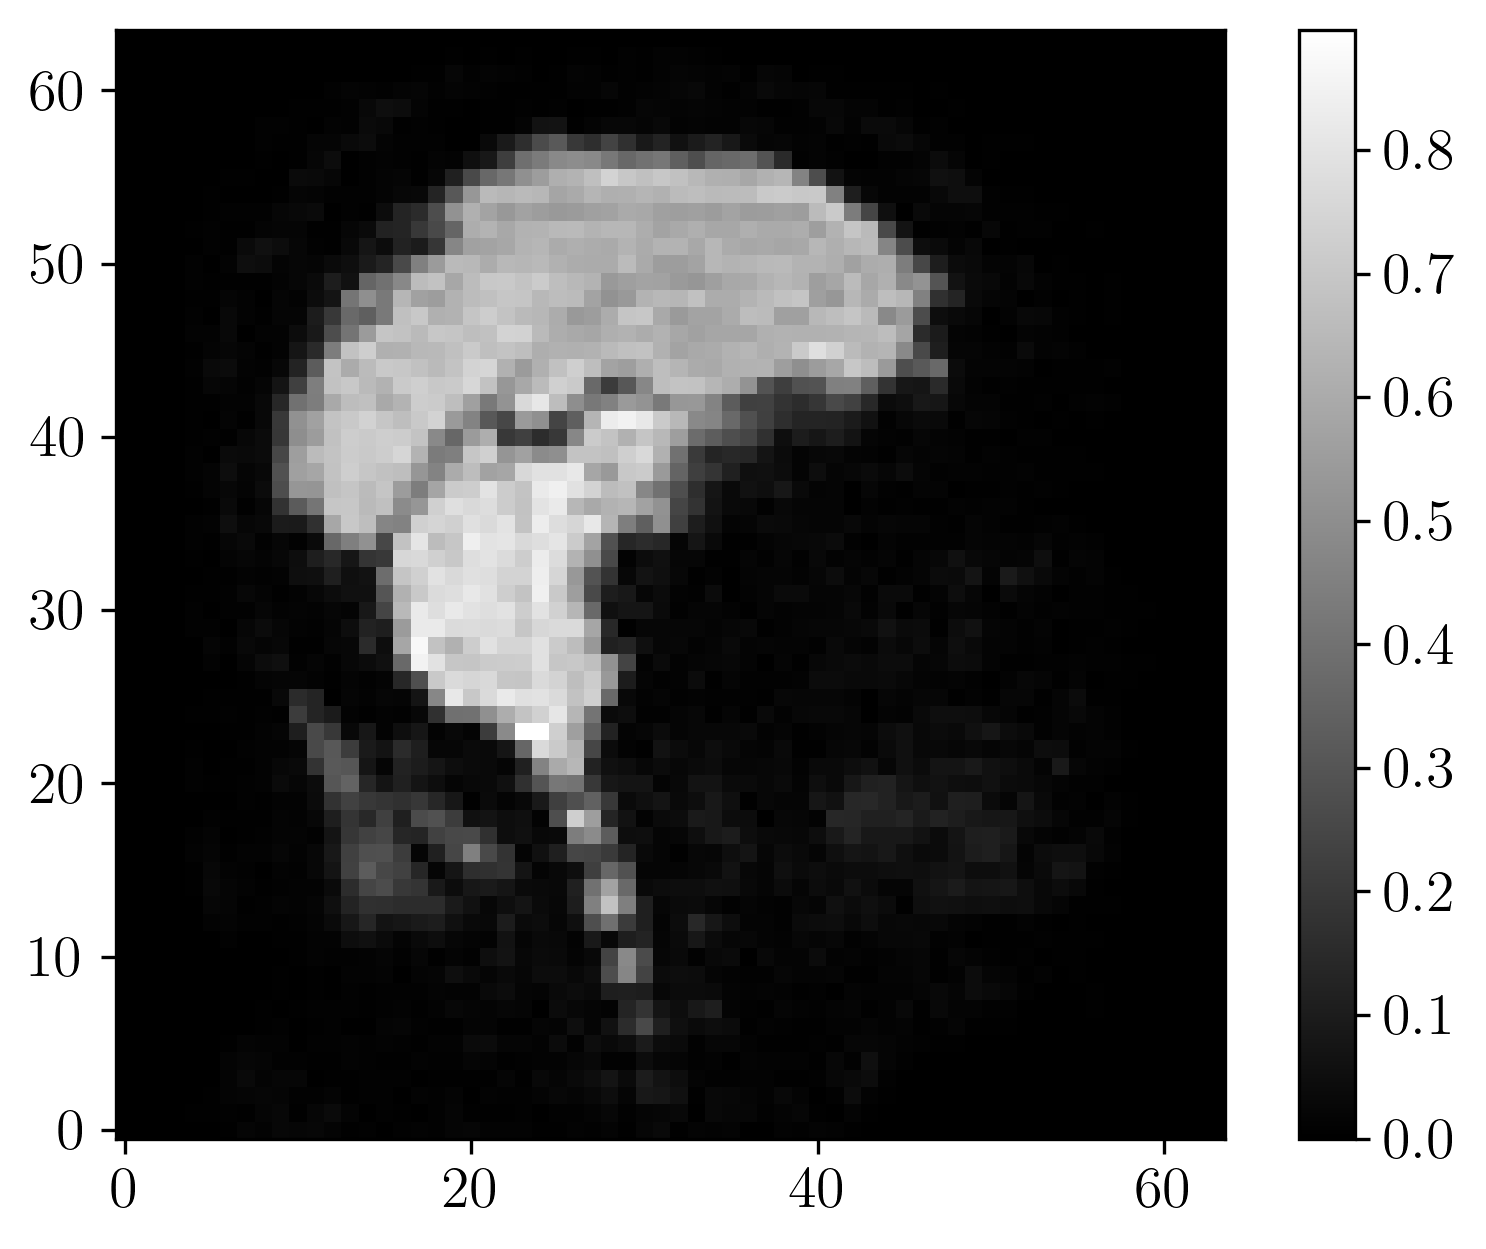
\includegraphics[width=0.33\textwidth]{images/fmri_forecasting/default/sub-07-5-1-1000-37-20-_-_-test.png}}}
	\hfill
	\subfloat[\fontsize{14pt}{14pt}\selectfont\centeringВосстановленный]{\label{fig:example-b}{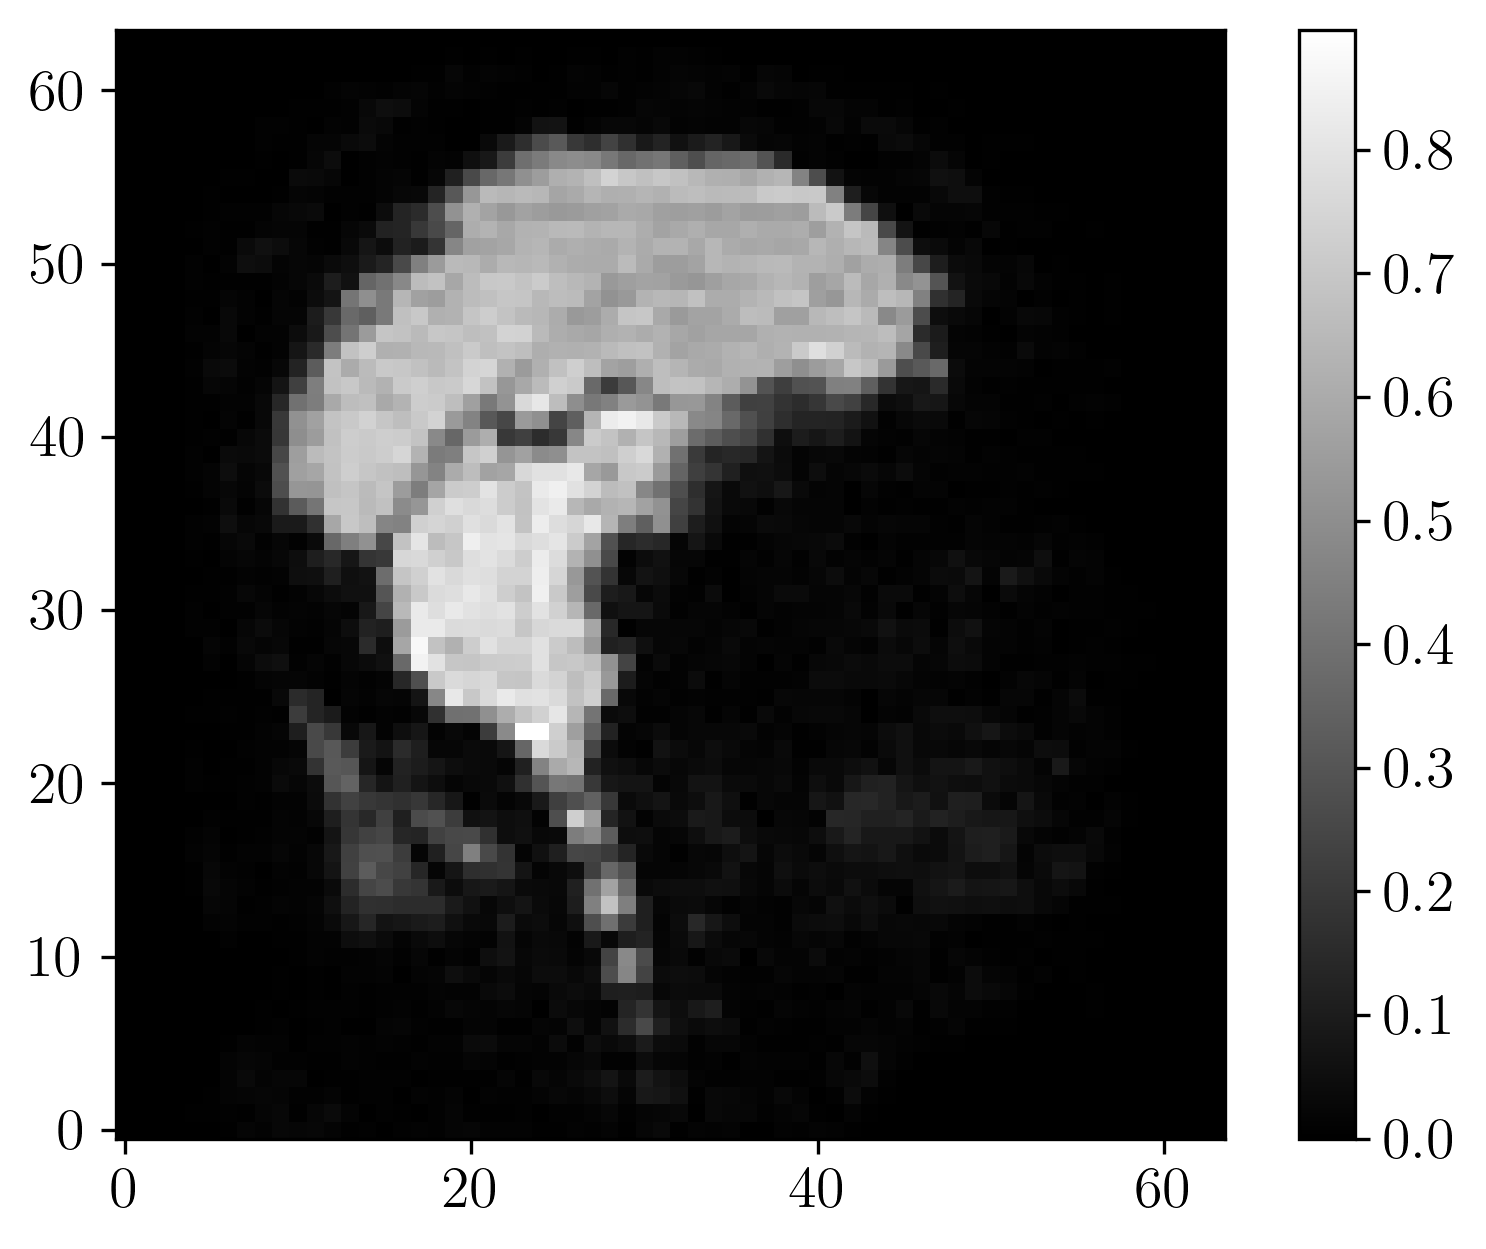
\includegraphics[width=0.33\textwidth]{images/fmri_forecasting/default/sub-07-5-1-1000-37-20-_-_-predicted.png}}}
	\hfill
	\subfloat[\fontsize{14pt}{14pt}\selectfont\centeringРазность]{\label{fig:example-c}{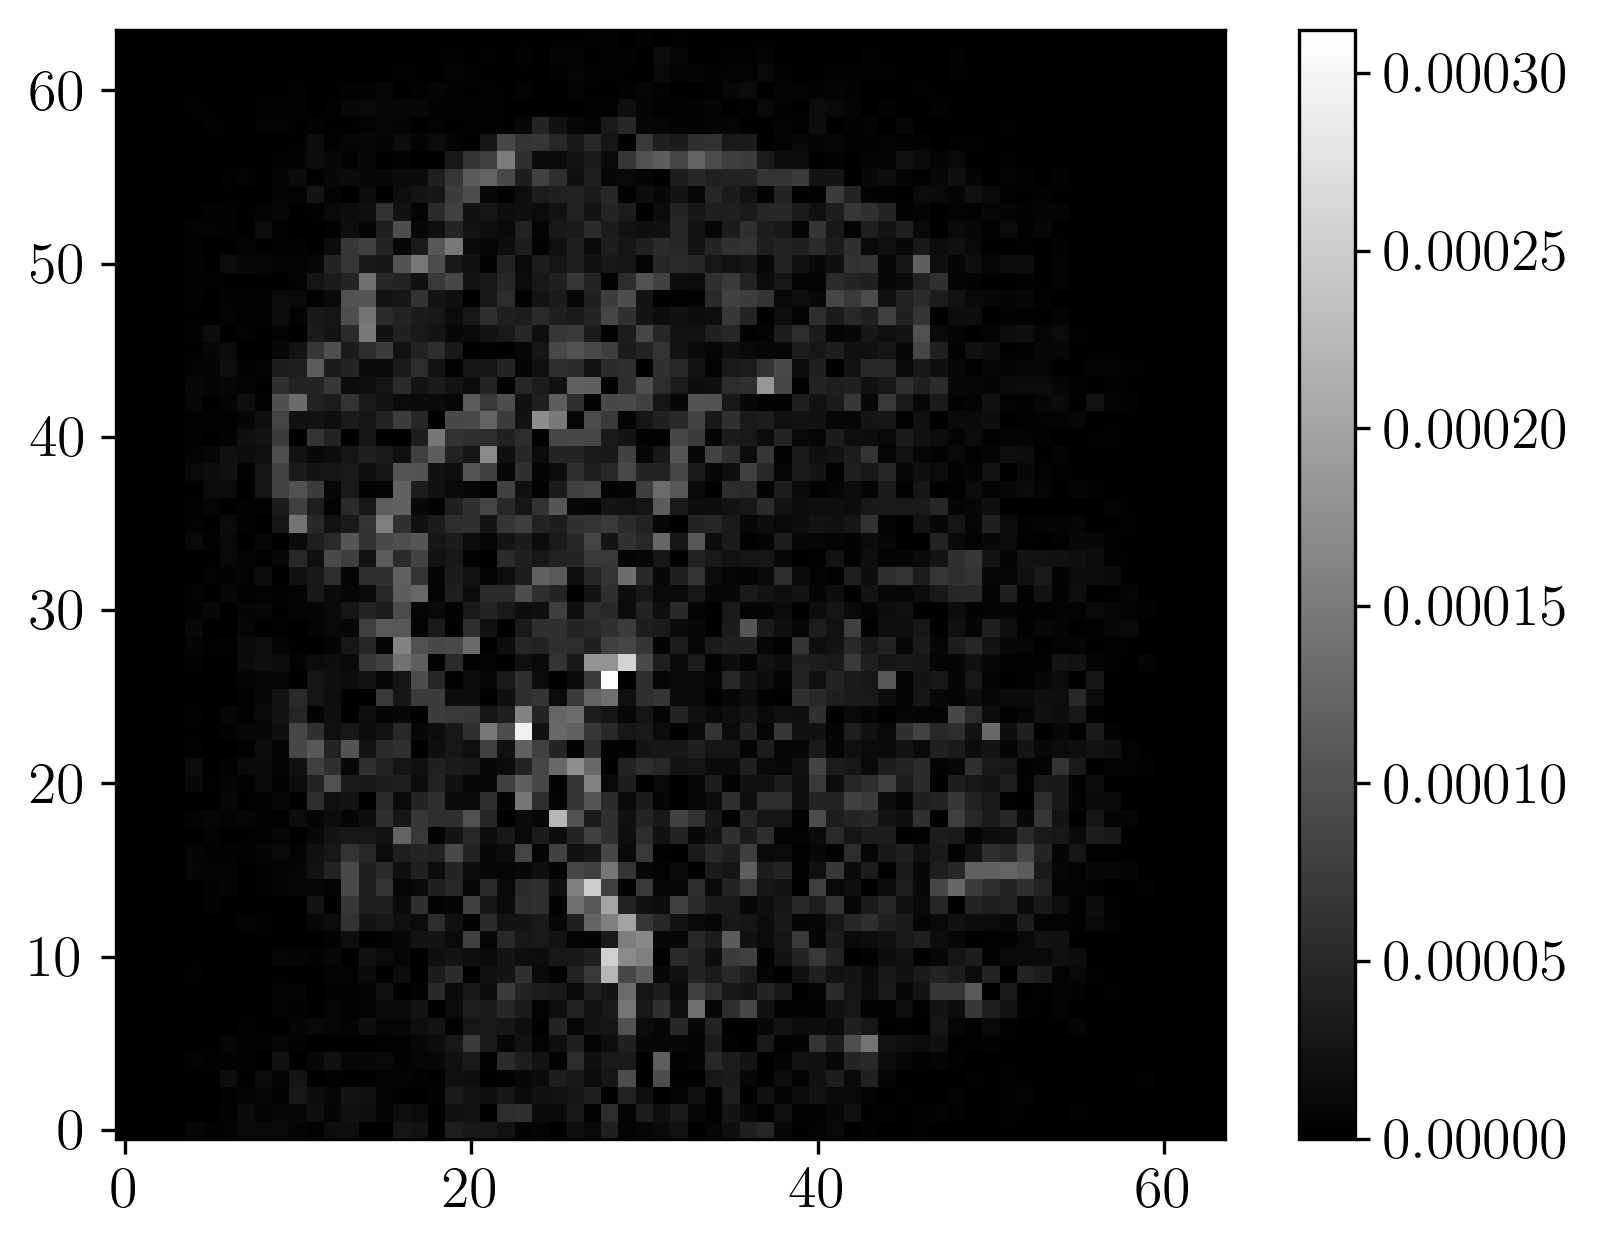
\includegraphics[width=0.33\textwidth]{images/fmri_forecasting/default/sub-07-5-1-1000-37-20-_-_-difference.png}}}
	\caption{Срез снимка фМРТ из тестовой выборки}
	\label{fig:example}
\end{figure}

\paragraph*{Анализ времени задержки.}

Исследована зависимость качества восстановления от времени задержки.
Для примера был выбран 47-ой испытуемый.
На левом графике Рис.~\ref{fig:mse-dt} представлена зависимость метрики MSE
от времени задержки $\Delta t$.
Исследование \citep{anderson2006} подтверждает, что наиболее активная часть мозга
при рассматриваемом обследовании~--- затылочная доля.
Остальные части вносят шум в рассматриваемую зависимость.
В настоящей работе проведена локализация вышеупомянутой области, 
что видно на Рис.~\ref{fig:local}.
Для локализации области отсекаются нижняя треть и правые две трети объемного
томографического изображения.
Красным цветом выделена та зона, в которую попадают 3\% наиболее 
изменяющихся вокселей затылочной доли.
Для этого все воксели локализованной области были упорядочены по 
убыванию суммарного абсолютного изменения значений.
Далее были выбраны 3\% вокселей с наибольшими изменениями.
Произведен пересчет метрики MSE именно на этой части снимка.
Соответствующий график приведен справа на Рис.~\ref{fig:mse-dt}.

\begin{figure}[h!]
	\centering
	\subfloat[\fontsize{14pt}{14pt}\selectfont\centeringИстинный]{\label{fig:local-a}{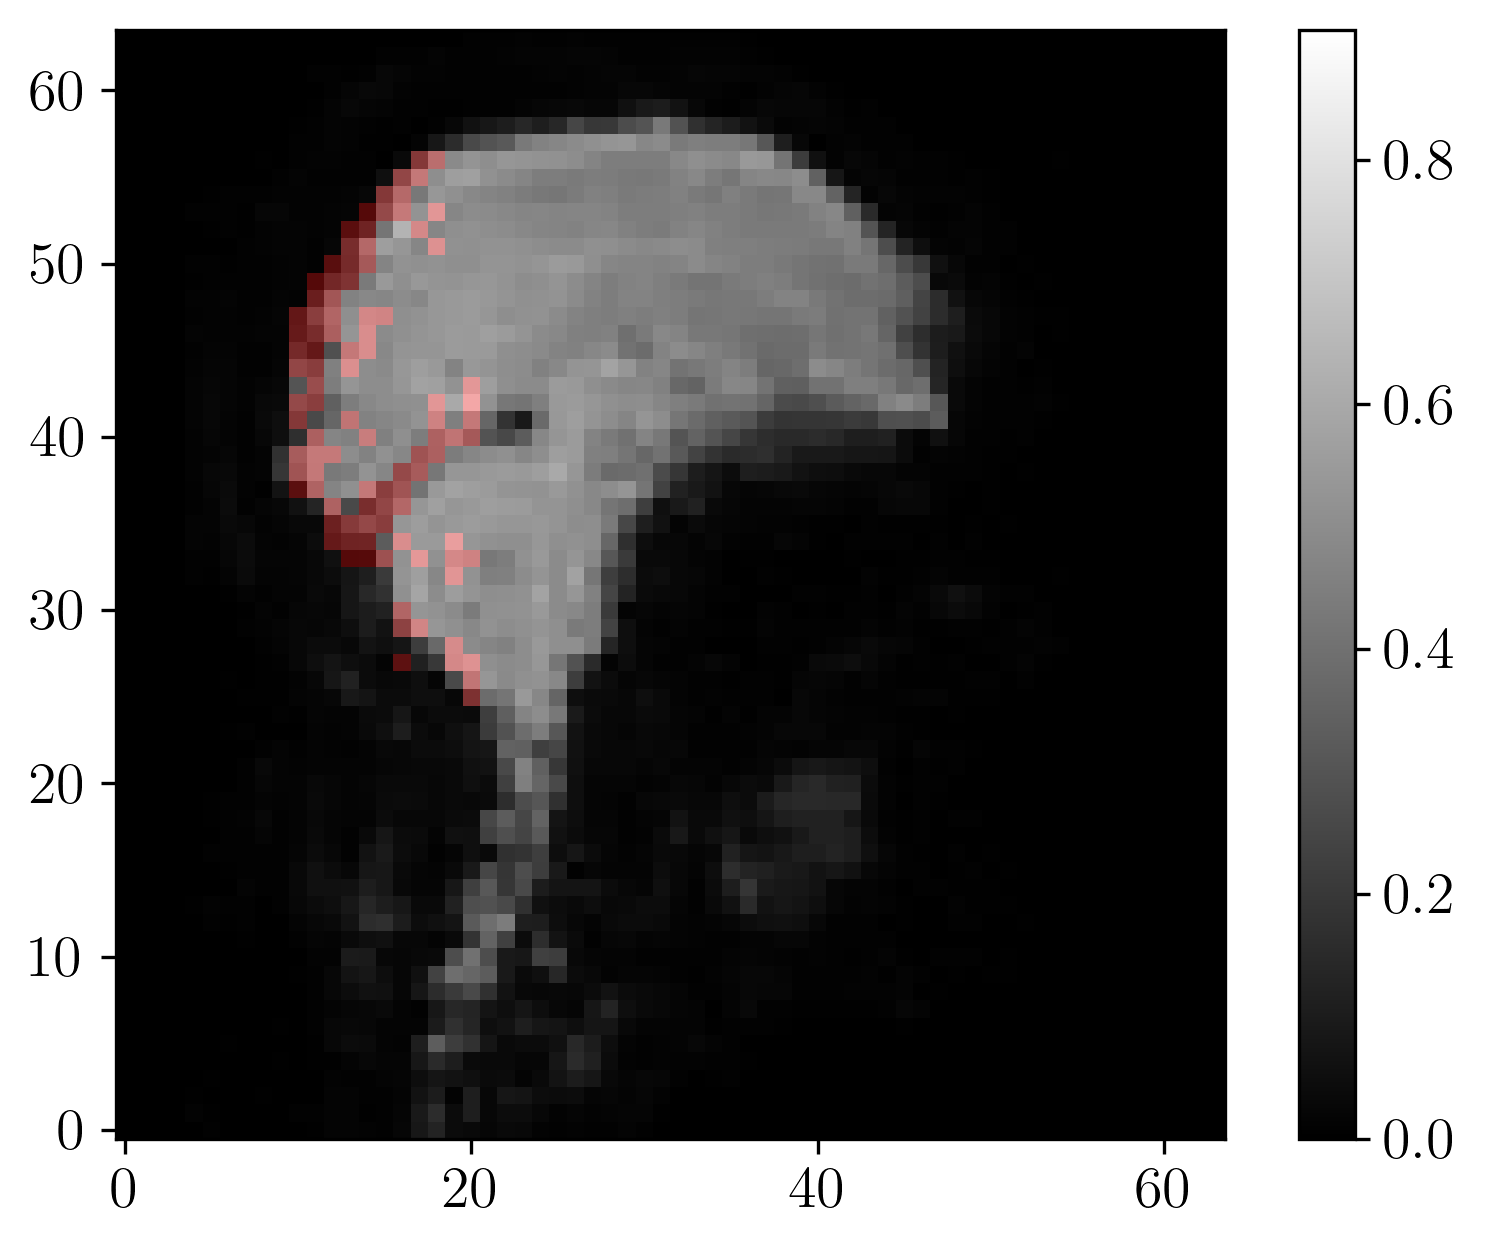
\includegraphics[width=0.33\textwidth]{images/fmri_forecasting/local/sub-47-5-1-1000-37-20-_-_-test.png}}}
	\hfill
    	\subfloat[\fontsize{14pt}{14pt}\selectfont\centeringВосстановленный]{\label{fig:local-b}{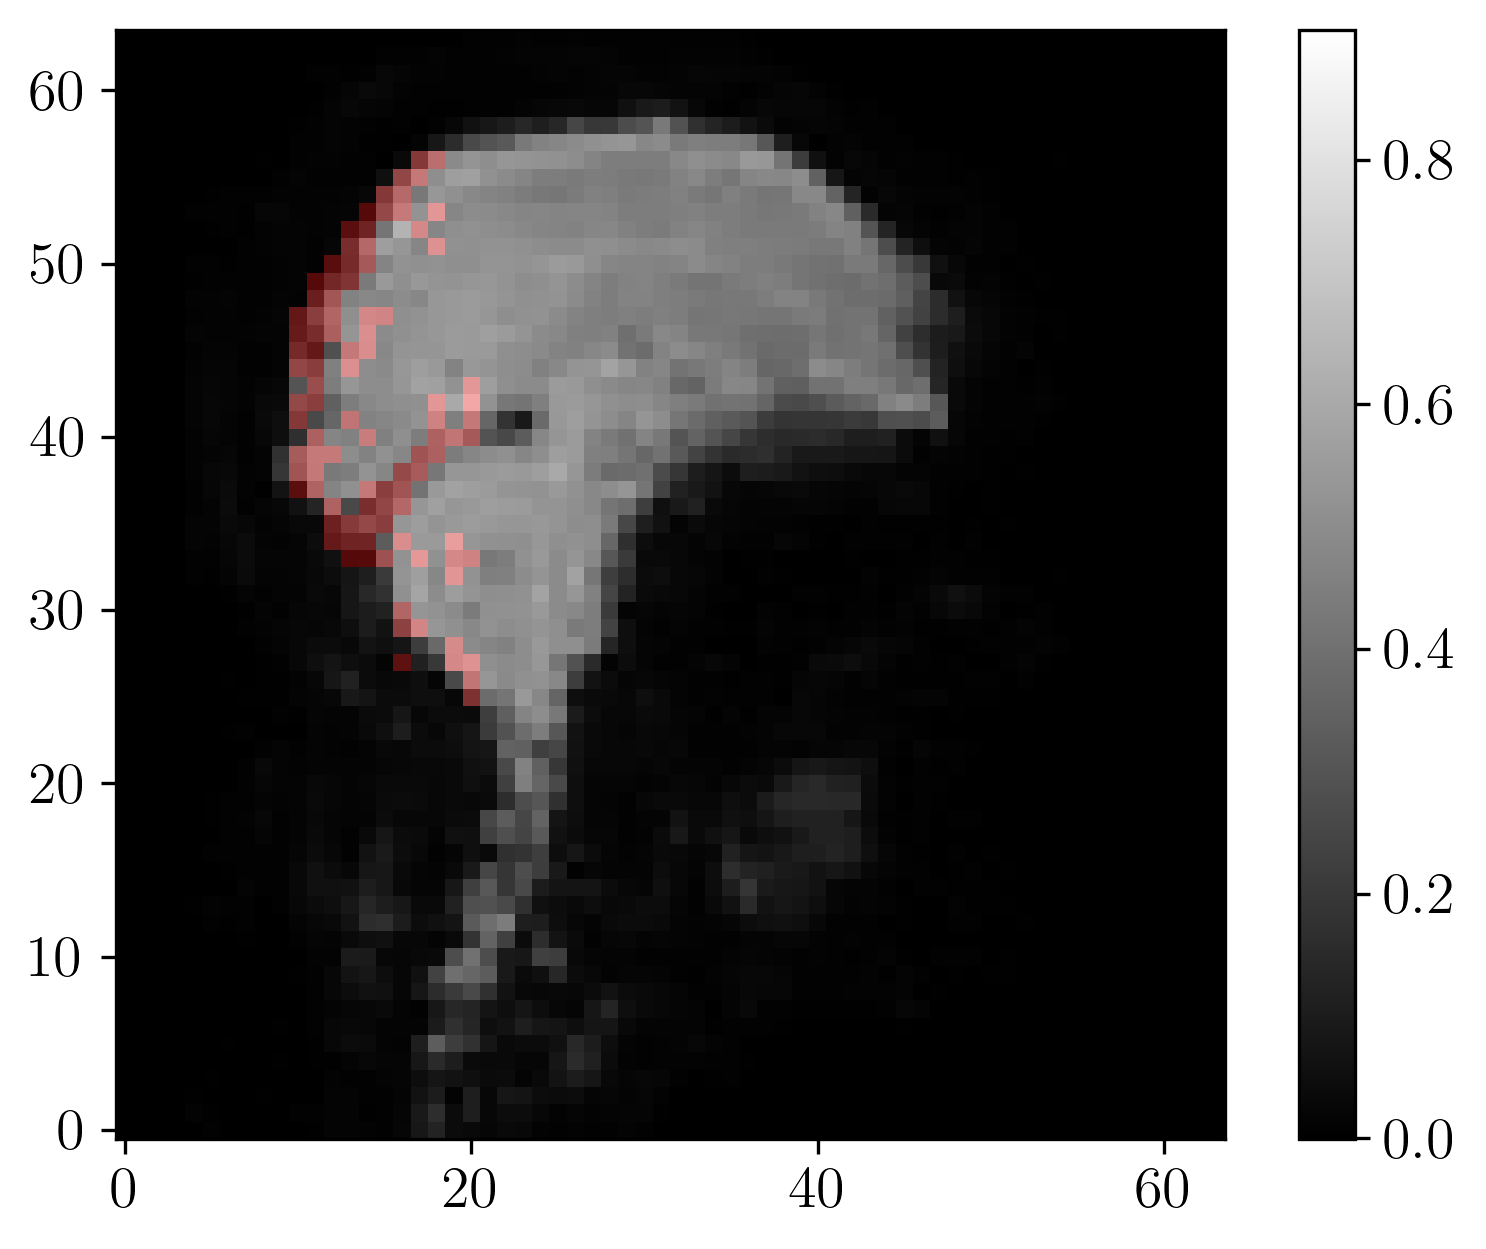
\includegraphics[width=0.33\textwidth]{images/fmri_forecasting/local/sub-47-5-1-1000-37-20-_-_-predicted.png}}}
	\hfill
	\subfloat[\fontsize{14pt}{14pt}\selectfont\centeringРазность]{\label{fig:local-c}{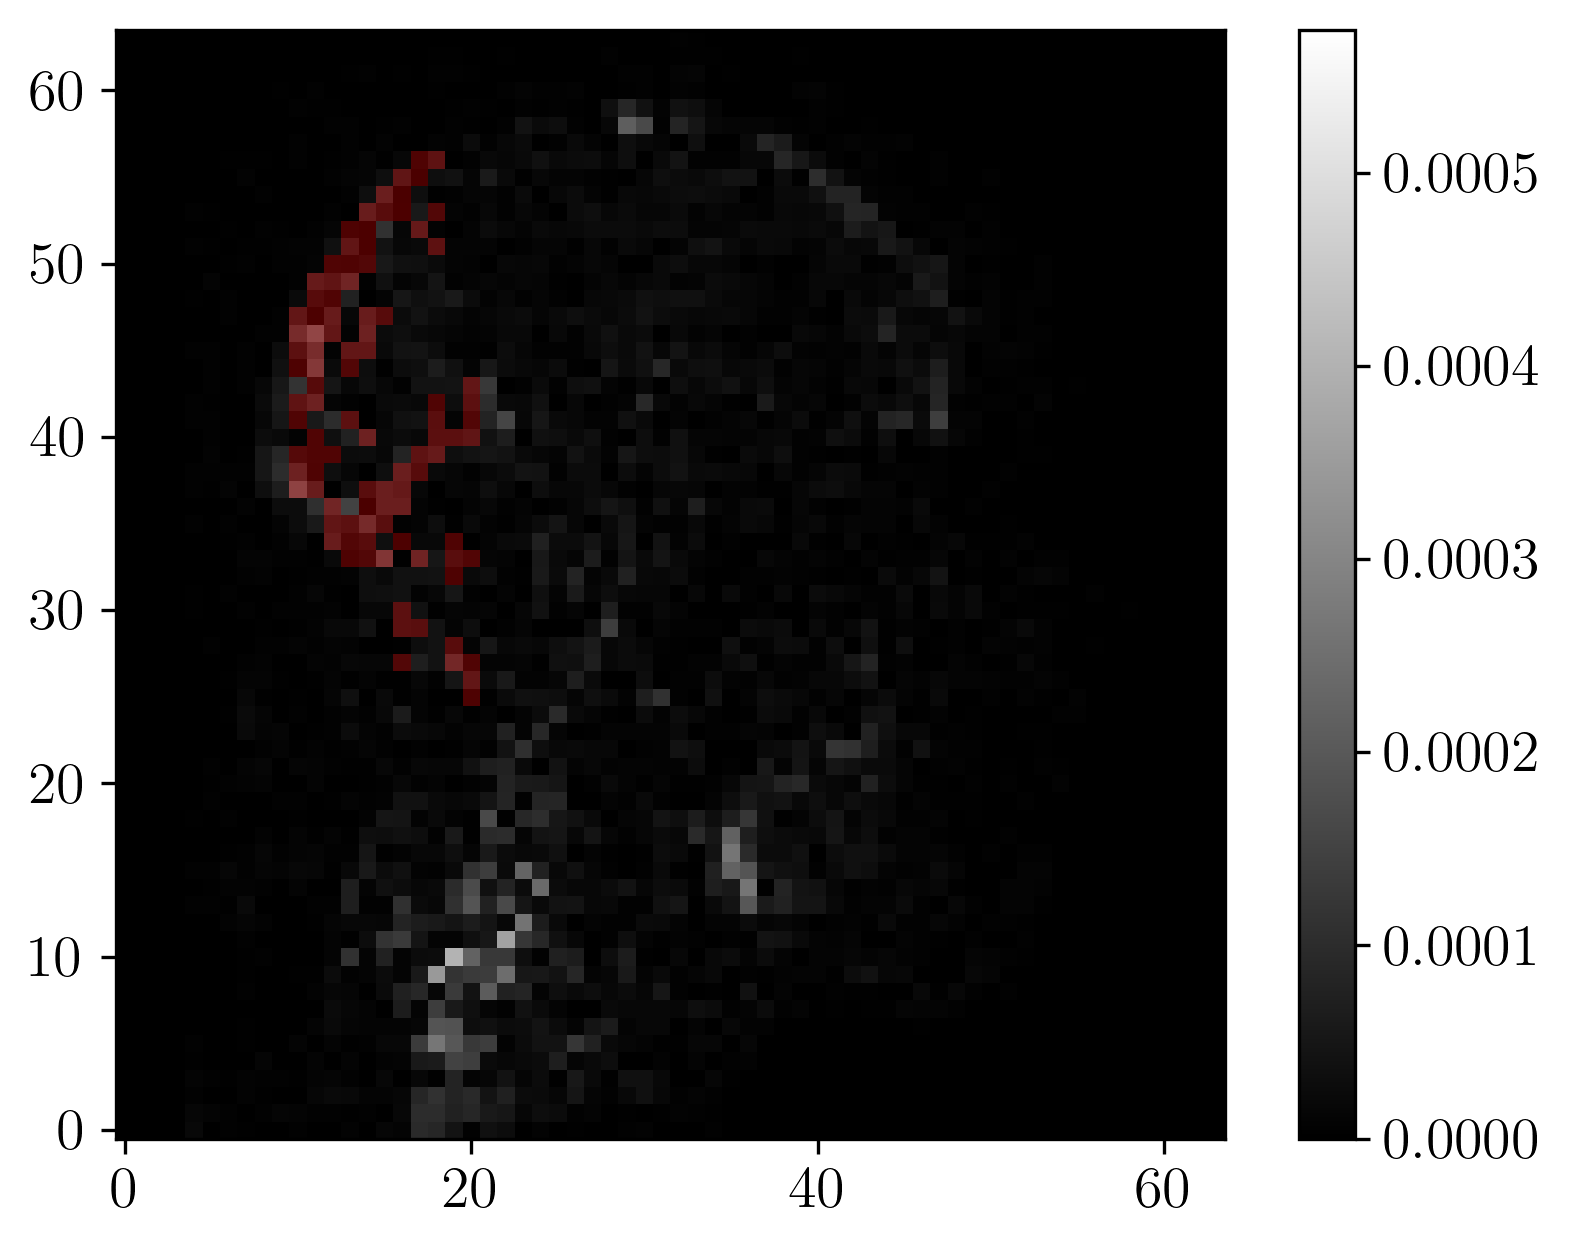
\includegraphics[width=0.33\textwidth]{images/fmri_forecasting/local/sub-47-5-1-1000-37-20-_-_-difference.png}}}
	\caption{Локализация наиболее активной зоны}
	\label{fig:local}
\end{figure}

\begin{figure}[h!]
	\centering
	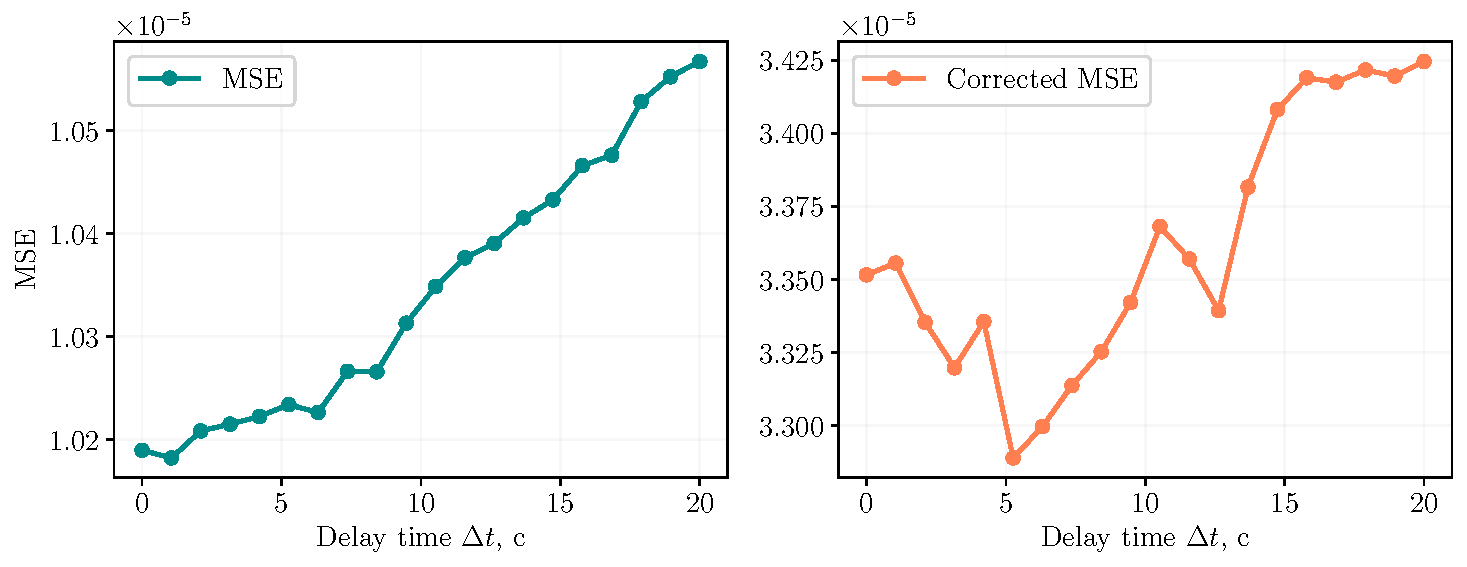
\includegraphics[width=\textwidth]{images/fmri_forecasting/mse_dt.pdf}
	\caption{Зависимость метрики MSE от времени задержки}
	\label{fig:mse-dt}
\end{figure}

\paragraph*{Подбор оптимального коэффициента регуляризации.}

Проведен анализ зависимости MSE от коэффициента регуляризации $\alpha$.
Рассматривались коэффициенты сжатия 1, 2, 4 и 8.
Соответствующие графики приведены на Рис.~\ref{fig:mse-alpha}.
Для построения графика производилось усреднение по испытуемым.
Обозначены границы среднеквадратичного отклонения.
Из графиков видно, что оптимальное значение коэффициента $\alpha \approx 1000$.
Вид кривой сохраняется независимо от коэффициента сжатия снимков фМРТ.

\begin{figure}[h!]
	\centering
	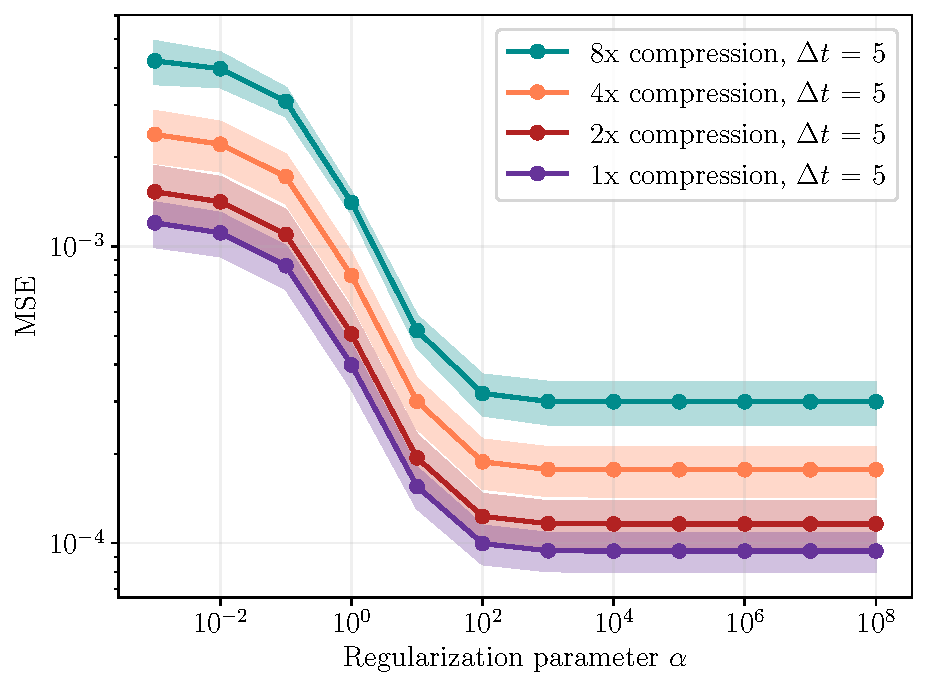
\includegraphics[width=0.65\textwidth]{images/fmri_forecasting/subs_MSE_alpha.pdf}
	\caption{Зависимость метрики MSE от коэффициента регуляризации $\alpha$ на снимках из тестовой выборки}
	\label{fig:mse-alpha}
\end{figure}

\paragraph*{Влияние коэффициента сжатия снимков на время работы метода.}

Производится сравнение времени обучения модели при использовании различных
коэффициентов сжатия снимков фМРТ. Рассматриваются коэффициенты 1, 2, 4 и 8.
Для каждого значения коэффициента сжатия подсчитывается среднее по всем испытуемым
значение времени обучения модели. Вычисляется среднеквадратичное отклонение.
Результаты эксперимента приведены в Таблице~\ref{table:coeffs}.
Время работы метода существенно уменьшается при использовании
предварительного сжатия снимков фМРТ. 
Эксперимент с подбором оптимального коэффициента регуляризации
подтверждает то, что сжатие снимков не изменяет вид зависимостей.

\begin{table}[h!]
	\centering
	\caption{Зависимость времени обучения модели от коэффициента сжатия}
	\begin{tabular}{|c|c|c|}
		\hline
		Коэффициент сжатия & Среднее время, с & Среднеквадратичное отклонение, с \\ \hline \hline
		1 & 36.3 & 6.1 \\ \hline
		2 & 6.7 & 0.5 \\ \hline
		4 & 1.6 & 0.1 \\ \hline
		8 & 1.4 & 0.3 \\ \hline
	\end{tabular}
	\label{table:coeffs}
\end{table}

\paragraph*{Анализ распределения весов модели.}

Построен график распределения значений компонент вектора весов модели.
Для построения производилось усреднение по всем вокселям для 4-го испытуемого.
Результат представлен на Рис.~\ref{fig:w-distr}.
Веса модели не лежат в окрестности какого-то конкретного значения, 
то есть их распределение не вырождено.
Этот результат вполне согласуется с реальностью, поскольку человек во время просмотра
обращает внимание на определенные части кадра, например, персонажей или
другие детали.

\begin{figure}[h!]
	\centering
	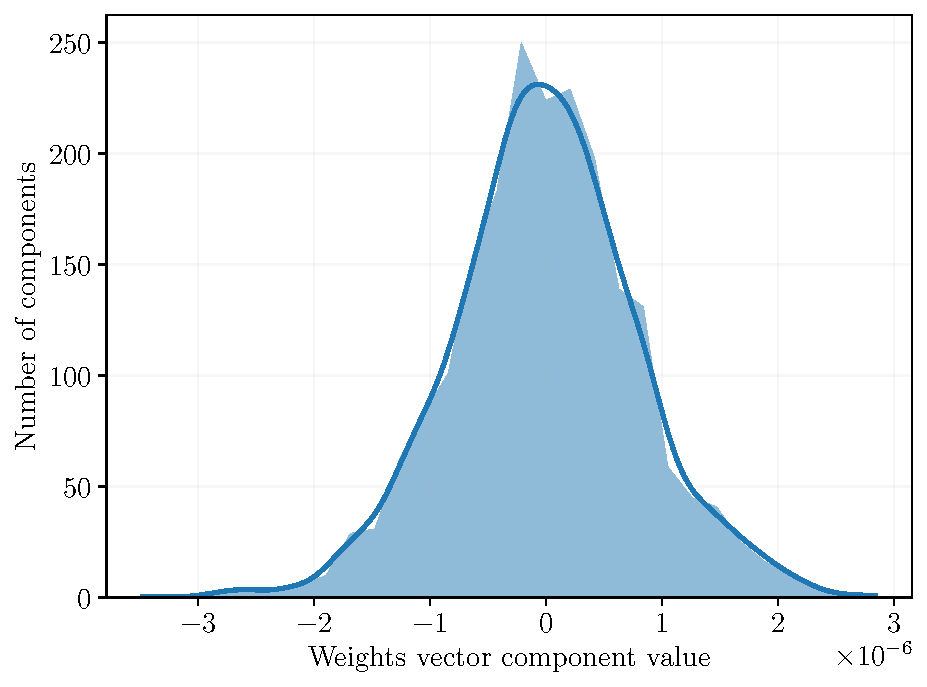
\includegraphics[width=0.65\textwidth]{images/fmri_forecasting/distribution.pdf}
	\caption{Распределение значений компонент вектора весов}
	\label{fig:w-distr}
\end{figure}

\paragraph*{Гипотеза инвариантности весов модели относительно человека.}

Проведена проверка гипотезы инвариантности весов модели относительно человека:
использование матрицы весов одного испытуемого для восстановления снимков фМРТ другого.
Использовалась метрика MSE на тестовой выборке.
Результаты представлены в Таблице~\ref{table:inv}.
Рассмотрены 4-ый и 7-ый испытуемые. Матрица весов 4-го использовалась для восстановления
снимков 7-го.
Значения MSE практически совпадают. 

\begin{table}[h!]
	\centering
	\caption{Проверка гипотезы инвариантности весов модели относительно человека}
	\begin{tabular}{|c|c|c|c|}
		\hline
		Матрица весов & Истинная             & Подмешанная  & Разность        \\ \hline \hline
		MSE           & $6.3912 \cdot 10^{-5}$ & $6.3911 \cdot 10^{-5}$ & $1.37 \cdot 10^{-9}$ \\ \hline
	\end{tabular}
	\label{table:inv}
\end{table}

Аналогичный эксперимент проведен для каждой пары испытуемых.
Полученные результаты представлены на Рис.~\ref{fig:heatmap},
который был получен следующим образом.
Рассматривается некоторый испытуемый (соответствует строке матрицы), 
для него вычисляется MSE~--- <<истинный>>.
Далее рассматривается другой испытуемый (соответствует столбцу матрицы),
берется его матрица весов, и с помощью нее делается предсказание для первого 
испытуемого, затем вычисляется MSE~--- <<подмешанный>>. 
Разность между полученными MSE в процентах от <<истинного>> заносится в матрицу.
Положительное значение означает, что <<подмешанный>> MSE больше, чем <<истинный>>.
Отрицательное~--- что <<подмешанный>> меньше.
Идеальная модель должна приводить только к положительным значениям отклонений, однако,
как видно из Рис.~\ref{fig:heatmap}, в матрице есть и отрицательные значения.
Тем не менее, они достаточно малы, а именно соответствуют отклонениям порядка 1\%.
Это объясняется тем, что модель достаточно простая, а потому обладает
высокой обобщающей способностью.
Однако это не мешает сделать вывод о том, что данные не противоречат гипотезе 
об инвариантности весов модели относительно человека.

\begin{figure}[h!]
	\centering
	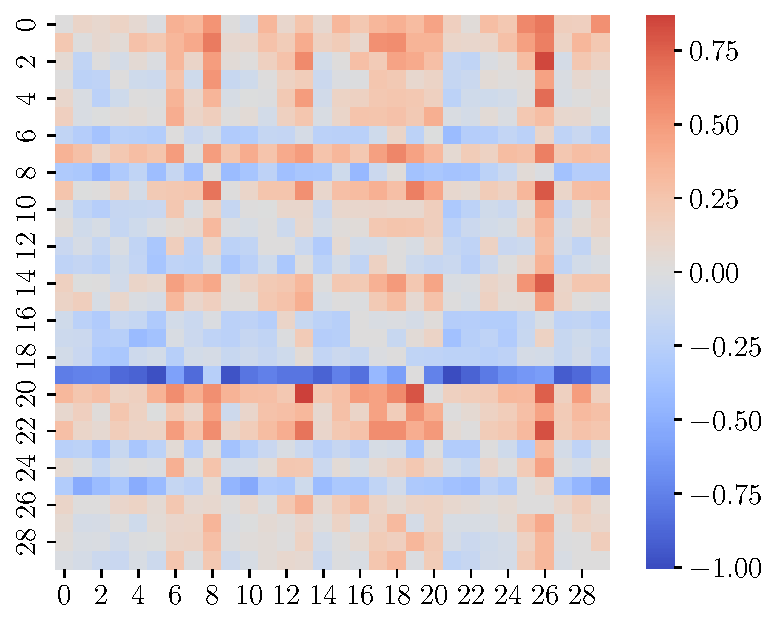
\includegraphics[width=0.5\textwidth]{images/fmri_forecasting/heatmap.pdf}
	\caption{MAPE изменения MSE при предсказании по подмешанной матрице весов (в процентах)}
	\label{fig:heatmap}
\end{figure}

\paragraph*{Корректность метода.}

Рассмотрено качество работы метода на неинформативных данных.
В качестве матрицы объекты-признаки $\bX$ взята матрица, целиком состоящая из единиц.
Произведено сравнение с результатами на настоящей матрице признакового описания.
К первому снимку 35-го испытуемого последовательно прибавляются все восстановленные
изменения значений вокселей.
В результате имеем последний снимок последовательности. На Рис.~\ref*{fig:recover}
представлены срезы последнего истинного и восстановленного снимков из тестовой выборки.
На Рис.\myfigref{fig:recover}{fig:recover-c} видна разность между ними.
Результаты на неинформативных продемонстрированы на Рис.~\ref{fig:random}.
Разность между истинным и восстановленным снимками при работе с неинформативными данными
значительно выше, что подтверждает наличие зависимости между показаниями датчиков и
изображениями из видеоряда. Численные результаты приведены в Таблице~\ref{table:random}.

\begin{figure}[h!]
	\centering
	\subfloat[\fontsize{14pt}{14pt}\selectfont\centeringИстинный]{\label{fig:recover-a}{\includegraphics[width=0.33\textwidth]{images/fmri_forecasting/original/sub-35-5-1-1000--1-20-_-_-recovered-test.png}}}
	\hfill
	\subfloat[\fontsize{14pt}{14pt}\selectfont\centeringВосстановленный]{\label{fig:recover-b}{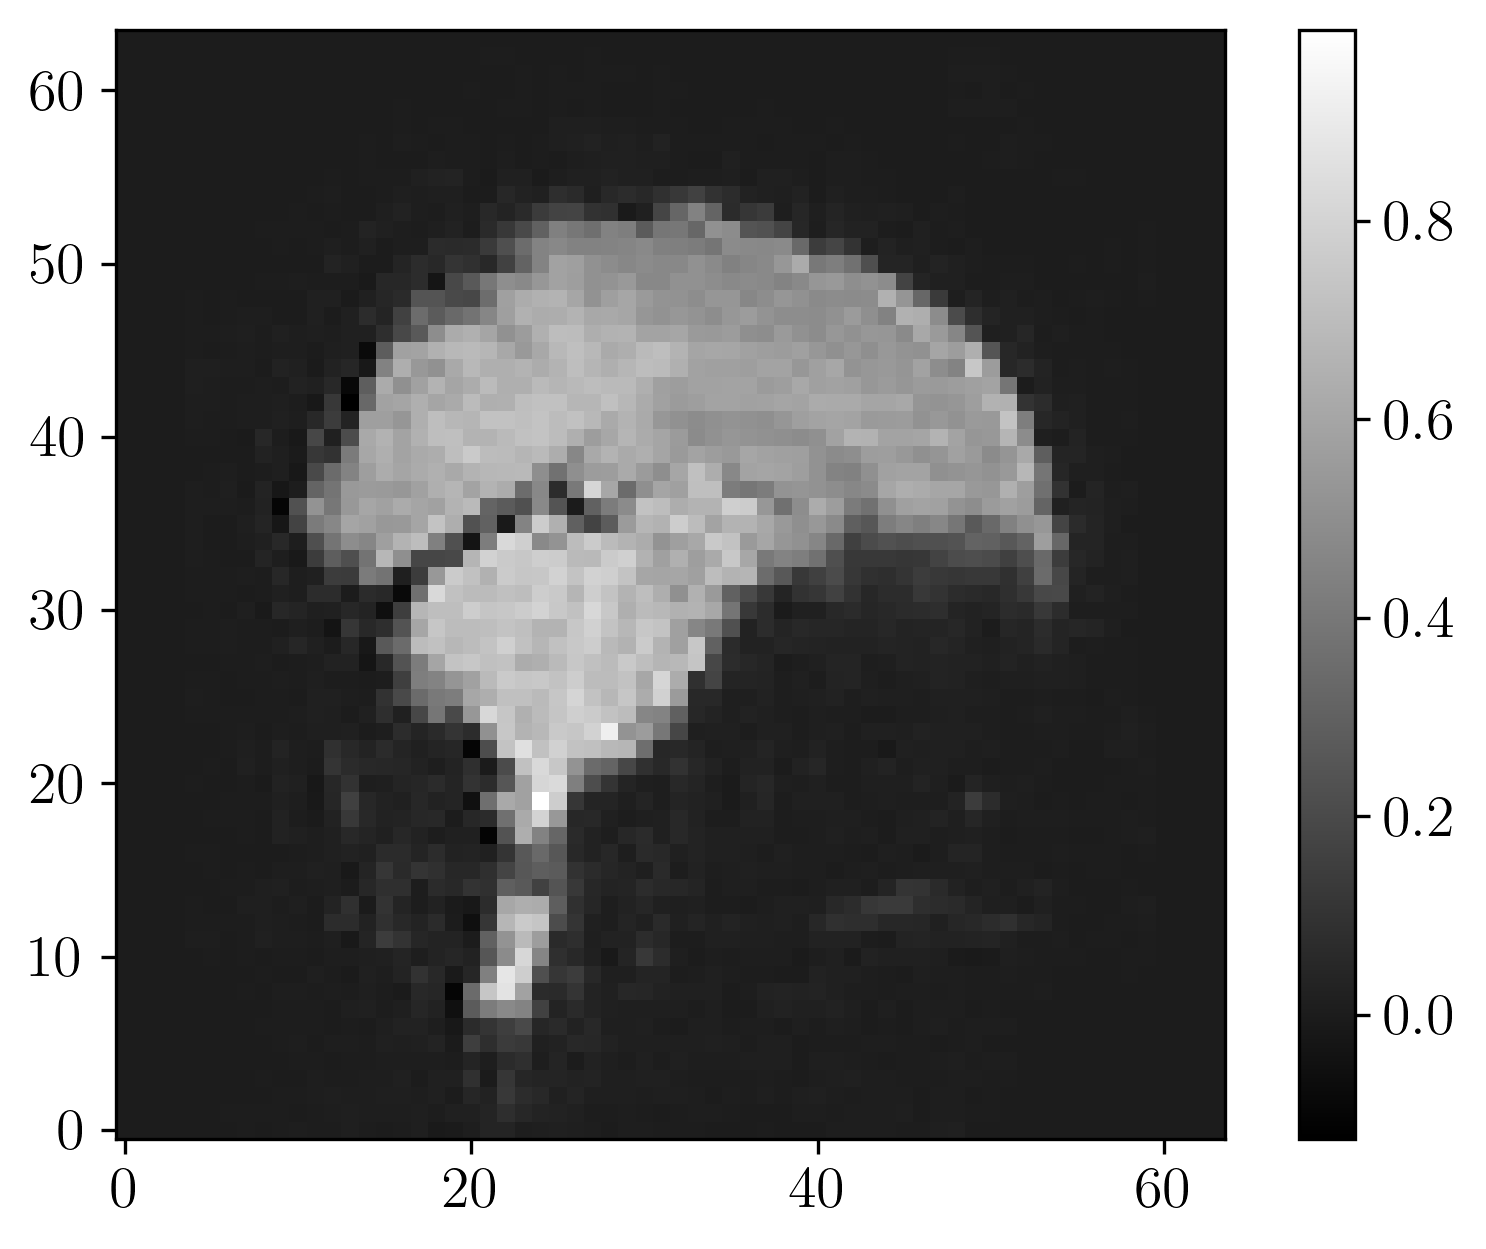
\includegraphics[width=0.33\textwidth]{images/fmri_forecasting/original/sub-35-5-1-1000--1-20-_-_-recovered-predicted.png}}}
	\hfill
	\subfloat[\fontsize{14pt}{14pt}\selectfont\centeringРазность]{\label{fig:recover-c}{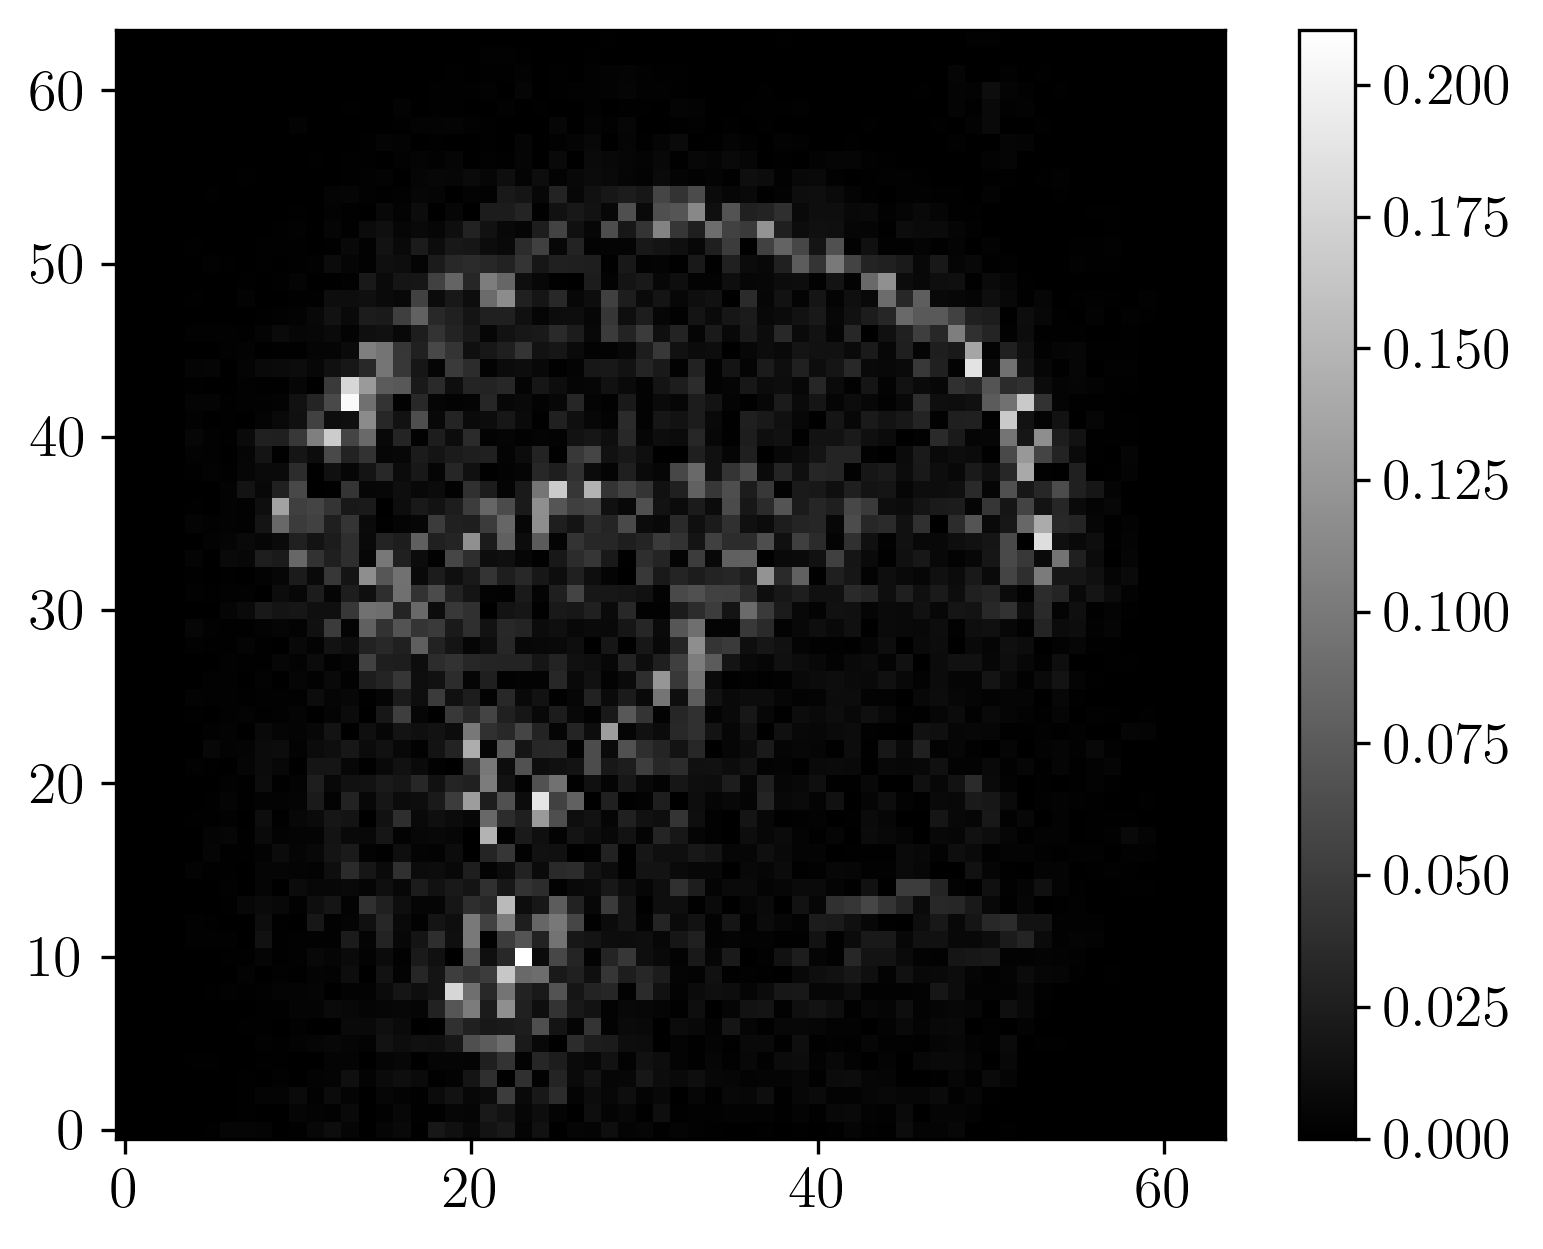
\includegraphics[width=0.33\textwidth]{images/fmri_forecasting/original/sub-35-5-1-1000--1-20-_-_-recovered-difference.png}}}
	\caption{Срез снимка фМРТ из тестовой выборки}
	\label{fig:recover}
\end{figure}

\begin{figure}[h!]
	\centering
	\subfloat[\fontsize{14pt}{14pt}\selectfont\centeringИстинный]{\label{fig:random-a}{\includegraphics[width=0.33\textwidth]{images/fmri_forecasting/noised/sub-35-5-1-1000--1-20-_-_-recovered-test.png}}}
	\hfill
	\subfloat[\fontsize{14pt}{14pt}\selectfont\centeringВосстановленный]{\label{fig:random-b}{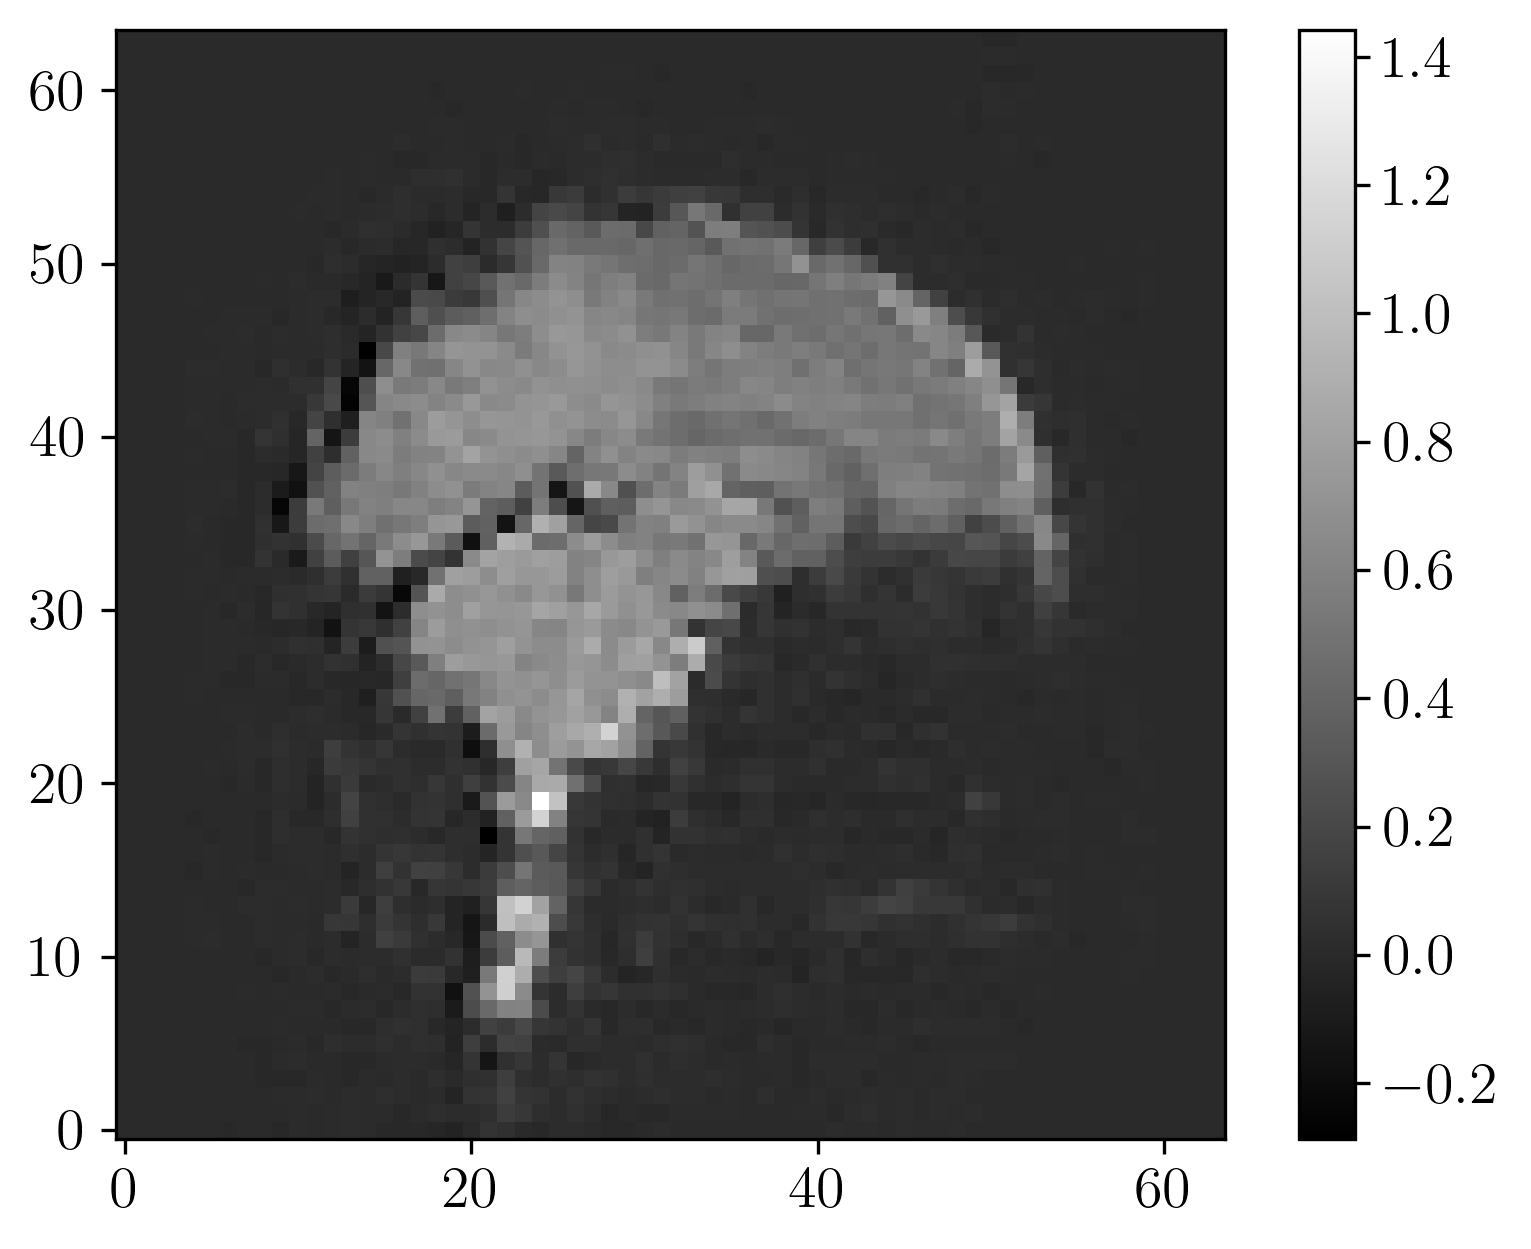
\includegraphics[width=0.33\textwidth]{images/fmri_forecasting/noised/sub-35-5-1-1000--1-20-_-_-recovered-predicted.png}}}
	\hfill
	\subfloat[\fontsize{14pt}{14pt}\selectfont\centeringРазность]{\label{fig:random-c}{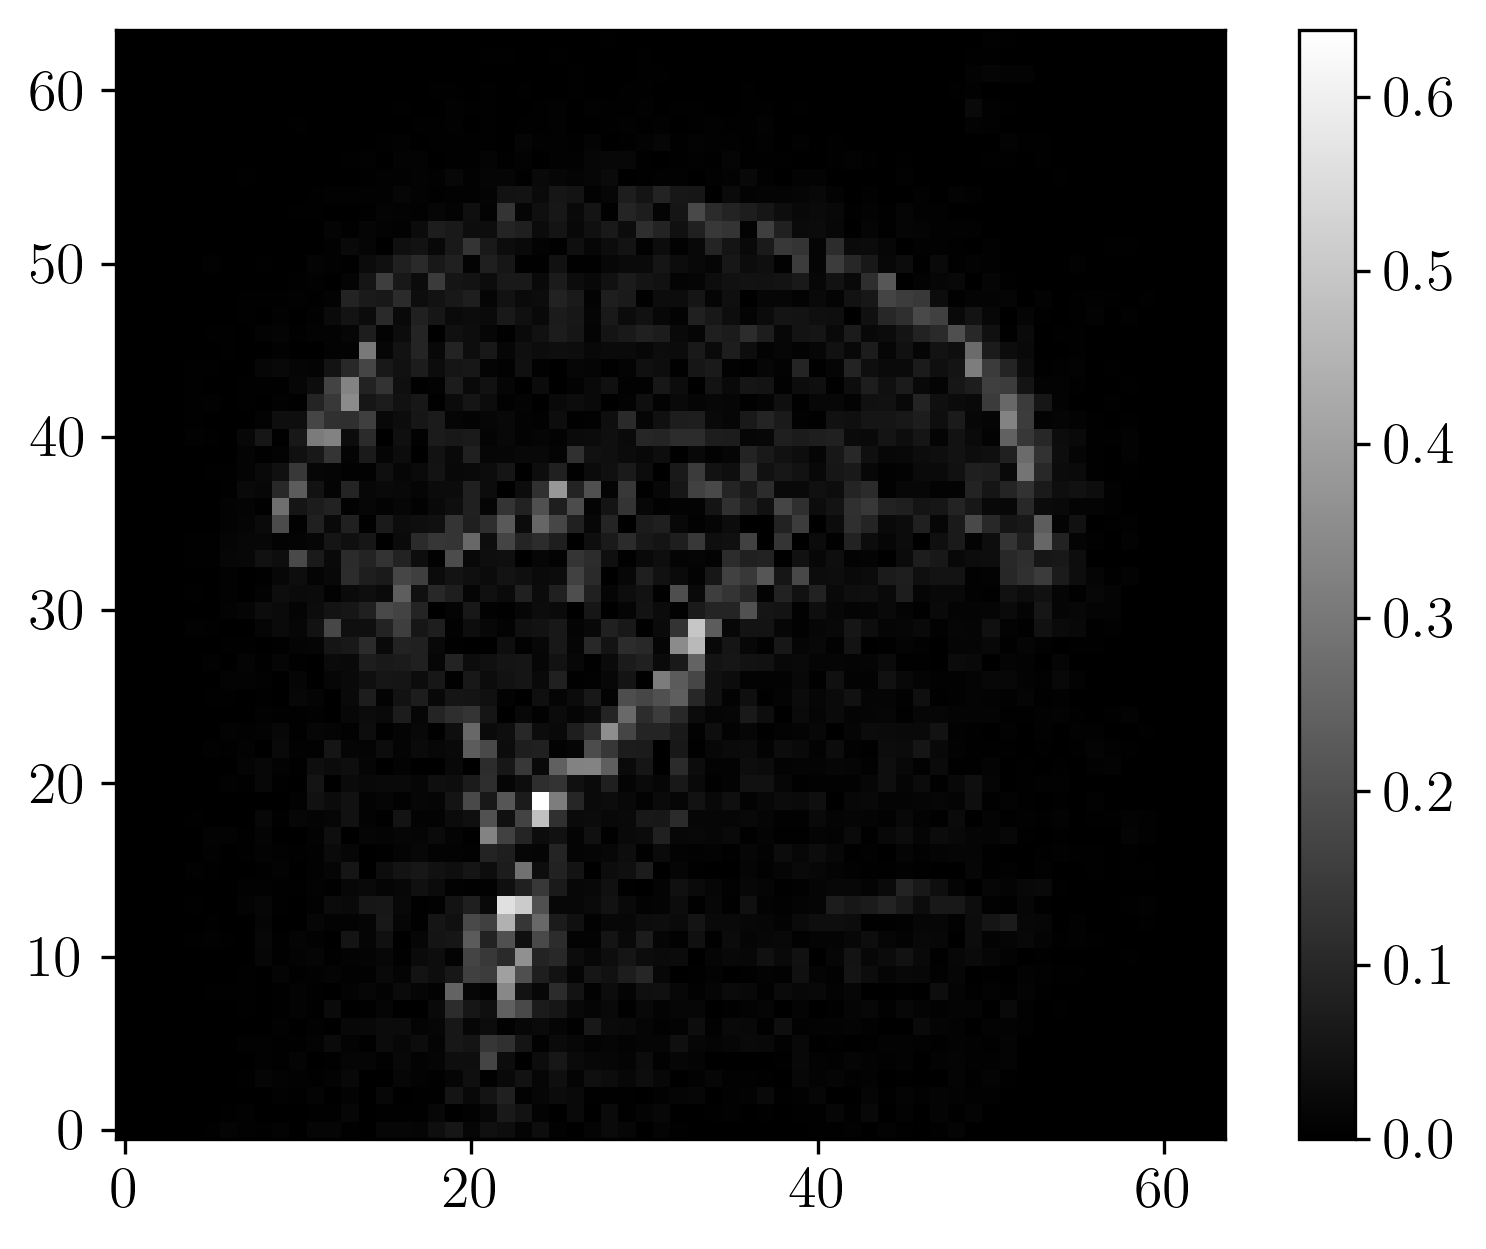
\includegraphics[width=0.33\textwidth]{images/fmri_forecasting/noised/sub-35-5-1-1000--1-20-_-_-recovered-difference.png}}}
	\caption{Срез снимка фМРТ из тестовой выборки (на неинформативных данных)}
	\label{fig:random}
\end{figure}

\begin{table}[h!]
	\centering
	\caption{Качество работы метода на неинформативных данных}
	\begin{tabular}{|c|c|c|c|}
		\hline
		Выборка & Истинная          & Неинформативные данные & Разность \\ \hline \hline
		MSE     & $3.67 \cdot 10^{-4}$ & $1.39 \cdot 10^{-3}$ & $1.02 \cdot 10^{-3}$ \\ \hline
	\end{tabular}
	\label{table:random}
\end{table}


\subsection{Взвешивание вокселей фМРТ снимков}
Для проведения вычислительного эксперимента используются данные фМРТ, собранные при изучении представлений лиц и объектов в вентральной височной коре. Набор данных впервые использовался в исследовании \cite{haxby2001distributed} и впоследствии стал известен как датасет Haxby. Данные широко используются в качестве сравнительной базы при изучении механизмов обработки визуальной информации в мозге.

Набор данных содержит показания фМРТ 6 испытуемых. Каждый испытуемый прошел 12 сеансов, в каждом из которых пассивно рассматривал черно-белые изображения восьми категорий, сгруппированные в блоки по 24 секунды, разделенные периодами отдыха. Каждое изображение демонстрировалось в течение 500 мс с последующим интервалом между стимулами 1500 мс. Данные фМРТ головного мозга были записаны с частотой 2.5 $\text{с}^{-1}$. Характеристики выборки приведены в Таблице~\ref{table:sample_2}.

\begin{table}[h!]
	\centering
	\caption{Описание выборки}
	\begin{tabular}{|c|c|c|}
		\hline
		Название                       & Обозначение & Значение             \\
		\hline \hline
		Количество снимков в сеансе & $\tau$ & 121 \\ \hline
		Частота снимков фМРТ           & $\mu$       & 2.5 $\text{с}^{-1}$ \\ \hline
		Размерности снимка             & $X, Y, Z$   & 40, 64, 64           \\ \hline
	\end{tabular}
	\label{table:sample_2}
\end{table}
Кроме того, набор данных содержит временные ряды стимулов и маски активных областей мозга, полученные нейробиологами. Эти области были определены для каждого участника эксперимента индивидуально. Маски активности были созданы путем объединения этих областей для всех участников эксперимента. 

\paragraph*{Демонстрация работы метода.}
Для демонстрации работы алгоритма был выбран 1-ый испытуемый, размер ядра $k_s = 4$, $h=10$. Рассмотрен 28-ой срез по первой координате.
Временной ряд стимула приведен в бинарный формат, где моменты наблюдения стимула отмечены единицей, а моменты отдыха~--- нулем.
На Рис.~\ref{fig:example1} представлены срезы снимка из выборки с соответствующими масками активности. На Рис.\myfigref{fig:example1}{fig:example-a} цветом отмечены области мозга, полученные методом \textit{Cross-Correlation Weighting}. На Рис.\myfigref{fig:example1}{fig:example-b} цветом показаны области мозга, полученные при статистическом анализе. Наконец, на Рис.\myfigref{fig:example1}{fig:example-c} цветом представлена разметка нейробиологов.

На основе \ref{par:stat_anal} экспериментально проверено, что корреляция областей мозга, полученных предложенным методом, со стимулом является статистически значимой. Кроме того, полученные области близки к разметке нейробиологов.

\begin{figure}[h!]
	\centering
	\subfloat[\fontsize{14pt}{14pt}\selectfont\centeringПредложенный метод]{\label{fig:example-a}{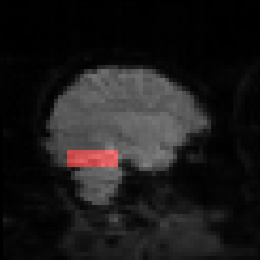
\includegraphics[width=0.3\textwidth]{images/fMRI_decoding/fmri_weighing/haxby_method.png}}}
	\hfill
	\subfloat[\fontsize{14pt}{14pt}\selectfont\centeringСтатистически значимые области]{\label{fig:example-b}{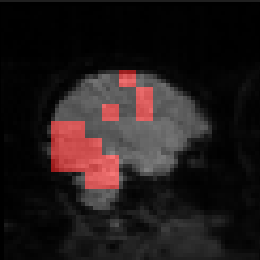
\includegraphics[width=0.3\textwidth]{images/fMRI_decoding/fmri_weighing/haxby_rejected.png}}}
	\hfill
	\subfloat[\fontsize{14pt}{14pt}\selectfont\centeringРазметка нейробиологов]{\label{fig:example-c}{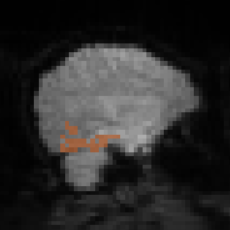
\includegraphics[width=0.3\textwidth]{images/fMRI_decoding/fmri_weighing/haxby_true.png}}}
 \caption{Взвешенные области мозга на срезе фМРТ снимка}
\label{fig:example1}
\end{figure}

\paragraph*{Корректность метода.} Рассмотрено качество работы метода на неинформативных данных. Используется временной ряд фМРТ 1-го испытуемого и случайно сгенерированный бинарный ряд стимула. На Рис.~\ref{fig:correctness} представлены срезы снимка фМРТ, цветом отмечены области мозга, предсказанные методом.

\begin{figure}[h!]
	\centering
	\subfloat{\label{fig:correctness-a}{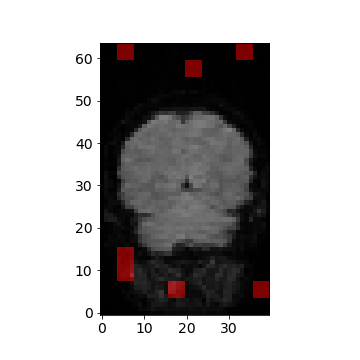
\includegraphics[width=0.33\textwidth]{images/fMRI_decoding/fmri_weighing/slice_dim_1_slice_20.png}}}
	\hfill
	\subfloat{\label{fig:correctness-b}{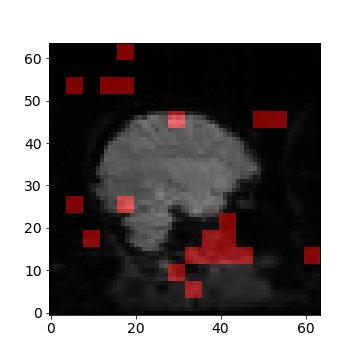
\includegraphics[width=0.33\textwidth]{images/fMRI_decoding/fmri_weighing/slice_dim_0_slice_28.png}}}
	\hfill
	\subfloat{\label{fig:correctness-c}{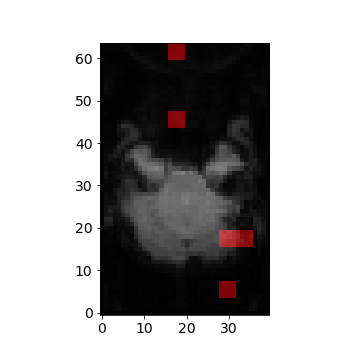
\includegraphics[width=0.33\textwidth]{images/fMRI_decoding/fmri_weighing/slice_dim_2_slice_24.png}}}
 \caption{Взвешенные области мозга, полученные по неинформативным данным}
\label{fig:correctness}
\end{figure}
Метод предсказывает случайные области, не имеющие отношения к активности головного мозга. 
На основе \ref{par:stat_anal} проверены гипотезы на значимость корреляции между выделенными областями и сгенерированным рядом стимула. Результаты статистического анализа не выявили значимости для какой-либо из полученных областей, что свидетельствует о наличии корреляции между активностью предсказанных областей мозга и истинным стимулированием.
\subsection{Классификация сегментов временного ряда фМРТ}
В рамках данного исследования проводится вычислительный эксперимент с использованием данных фМРТ Haxby. Рассматриваются данные фМРТ первого и второго испытуемого. Для получения сегментов ряда фМРТ был применен алгоритм сегментации, описанный в разделе \ref{segmentation}

В Таблице~\ref{table:sample_3} приведены параметры, рассчитанные для каждой из двух выборок, полученных в результате сегментации.
\begin{table}[h!]
	\centering
	\caption{Описание выборок, полученных в результате сегментации}
	\begin{tabular}{|c|c|c|}
		\hline
		Название                       & Обозначение & Значение             \\
		\hline \hline
		Число объектов & $N$ & 96 \\ \hline
		  Длина каждого сегмента           & $\tau$       & 19 \\ \hline
	   Число классов стимула             & $C$   & 8          \\ \hline
        Число объектов на каждый класс             & $N_k$   & 12         \\ \hline   
	\end{tabular}
	\label{table:sample_3}
\end{table} 

Произведено разделение каждой выборки на тренировочную и тестовую в соотношении $80\%$ к $20\%$ соответственно. Для оценки качества классификации сегментов фМРТ использовались метрики Accuracy, Macro-averaged F1 score и Micro-averaged F1 score.

В ходе экспериментов фиксировались следующие параметры предложенного метода: число выделяемых областей для каждого класса $h_k = 10,~k=1,\ldots, C$, размер ядра $k_s = 4$. Использовалась логистическая регрессия со стратегией <<один против всех>> и единичным коэффициентом $l2$-регуляризации. Кроме того, рассмотрен перцептрон, содержащий два скрытых слоя с размером, равным 100, и сигмоидной функцией активации.

В таблице~\ref{results} представлены усредненные значения метрик, полученные с помощью предложенного метода для двух испытуемых. 
\begin{table}[h!]
	\centering
	\caption{Среднее арифметическое метрик по испытуемым}
	\begin{tabular}{|c|c|c|c|}
		\hline
		Классификатор & Accuracy &  Macro F1 score & Micro F1 score\\
		\hline \hline
		Логистическая регрессия & 0.600 & 0.558 & 0.600\\ \hline  
          Перцептрон  & 0.700 & 0.636 & 0.636\\ \hline 
	\end{tabular}
	\label{results}
\end{table} 
Недостаточный объем выборки и большое число классов являются основными причинами переобучения и низких значений метрик. Тем не менее, у метода есть потенциал, на отдельных классах качество неплохое.

Для сравнения с предложенным методом классификации используются две упрощенные модели:
\begin{enumerate}
    \item В первой моделе отсутсвует векторизация с помощью \textit{Tangent Space Mapping}. После применения масок каждого класса временные ряды выпрямляются в вектор, конкатенируются и подаются на классификатор. Рассмотрены такие классификаторы, как логистическая регрессия и перцептрон.
    \item Во второй моделе отсутсвует шаг с подсчетом масок активности для каждого класса стимула. Маска подсчитывается аналогичным образом, но уже всреднем по всем временным рядам без учета категорий стимула. Кроме того, после применения маски используется векторизация с помощью \textit{Tangent Space Mapping}. Рассмотрены аналогичные первой модели классификаторы.
\end{enumerate}
В Таблице~\ref{comperison} представлены результаты работы трех методов на данных второго испытуемого. В качестве классификатора рассмотрена логистическая регрессия.
\begin{table}[h!]
	\centering
	\caption{Влияние отдельных компонент метода на качество классификации}
	\begin{tabular}{|c|c|c|c|}
		\hline
		Метод & Accuracy &  Macro F1 score & Micro F1 score\\
		\hline \hline
		Предложенный & 0.650 & 0.598 & 0.650\\ \hline  
           Без \textit{Tangent Space Mapping} & 0.150 & 0.121 & 0.150\\ \hline 
           Без масок активности & 0.400 & 0.376 & 0.400\\ \hline 
	\end{tabular}
	\label{comperison}
\end{table} 
После проведения анализа влияния различных компонентов модели на ее эффективность, было выявлено, что наибольшее снижение метрик происходит при исключении проекции на риманово касательное пространство. Кроме того, качество классификации также ухудшается, если не извлекаются маски активности для каждого класса стимула, а используется общая усредненная маска.
Данные результаты свидетельствуют о том, что пространственно-временные характеристики, такие как проекция на риманово касательное пространство и маски активности, играют важную роль в задаче декодирования нейронной активности. 